%%%% using 'arara' 4.0
% arara: xelatex: {synctex: yes, interaction: nonstopmode}
% arara: bibtex
% arara: xelatex: {synctex: yes, interaction: nonstopmode}
% arara: xelatex: {synctex: yes, interaction: nonstopmode}

% arara: indent: {overwrite: yes}

% arara: clean: { extensions: [aux, bcf, cod, blg, lof, lot, out, toc, log, xml, bak0 ] }

\documentclass[review]{elsarticle}

% Figures Links, mittig und rechts platzieren
\usepackage[export]{adjustbox}
\usepackage{caption}
\usepackage{subcaption}
\usepackage{amsmath}

% prevents that appendices are moved behind references
\usepackage{placeins}

\usepackage[nolist]{acronym}

\usepackage{longtable}
\usepackage{booktabs}
\usepackage{multirow}
\usepackage{float}

% enable linking to subsubsection
\setcounter{secnumdepth}{3}

% various symbols, e.g. \degree
\usepackage{gensymb}

\usepackage[hidelinks]{hyperref}

\usepackage{lineno}
\modulolinenumbers[5]

% set autoref abbr for appendix
\newcommand*{\Appendixautorefname}{appendix}

\journal{Journal "Remote Sensing of Environment"}

% line breaks in table cells
\newcommand{\specialcell}[2][l]{%
  \begin{tabular}[#1]{@{}l@{}}#2\end{tabular}}

% tilde
\newcommand{\mytilde}{\raise.17ex\hbox{$\scriptstyle\mathtt{\sim}$}}

%% APA style
\bibliographystyle{model5-names}\biboptions{authoryear}

\begin{document}

\begin{frontmatter}

	\title{title}

	%% Group authors per affiliation:
	\author[FSU]{Patrick Schratz}
	\cortext[mycorrespondingauthor]{Corresponding author}
	\ead{patrick.schratz@uni-jena.de}

	\author[FSU]{Jannes Muenchow}
	\author[NEIKER]{Eugenia Iturritxa}
	%\author[TUDO]{Jakob Richter}
	\author[FSU]{Alexander Brenning}

	\address[FSU]{Department of Geography, GIScience group, Grietgasse 6, 07743, Jena, Germany}
	%\address[NEIKER]{NEIKER, Granja Modelo –Arkaute, Apdo. 46, 01080 Vitoria-Gasteiz, Arab, Spain}
	%\address[TUDO]{Department of Statistics, TU Dortmund University, Germany}

	\begin{abstract}

	\end{abstract}

	\begin{keyword}
		hyperspectral imagery \sep statistical learning \sep spatial cross-validation
	\end{keyword}

\end{frontmatter}

\linenumbers

% längste Abkürzung steht hier!!! in eckigen Klammern
\begin{acronym}[AUROC]

	% geringerer Zeilenabstand
	%\setlength{\itemsep}{-\parsep}
	\acro{ANN}{Artificial Neural Network}
	\acro{AUROC}{Area Under the Receiver Operating Characteristics Curve}
	\acro{BRT}{Boosted Regression Trees}
	\acro{CART}{Classification and Regression Trees}
	\acro{CV}{cross-validation}
	\acro{ENM}{Environmental Niche Modeling}
	\acro{FPR}{False Positive Rate}
	\acro{GAM}{Generalized Additive Model}
	\acro{GBM}{Gradient Boosting Machine}
	\acro{GLM}{Generalized Linear Model}
	\acro{ICGC}{Institut Cartografic i Geologic de Catalunya}
	\acro{IQR}{Interquartile Range}
	\acro{WKNN}{Weighted $k$-nearest neighbor}
	\acro{MARS}{Multivariate Adaptive Regression Splines}
	\acro{MEM}{Maximum Entropy Model}
	\acro{NRI}{Normalized Ratio Index}
	\acro{OLS}{Ordinary Least Squares}
	\acro{LOWESS}{Locally Weighted Scatter Plot Smoothing}
	\acro{PISR}{Potential Incoming Solar Radiation}
	\acro{RBF}{Radial Basis Function}
	\acro{RF}{Random Forest}
	\acro{RMSE}{Root Mean Square Error}
	\acro{RR}{Ridge Regression}
	\acro{RSS}{Residual Sum of Squares}
	\acro{SDM}{Species Distribution Modeling}
	\acro{SVM}{Support Vector Machines}
	\acro{TPR}{True Positive Rate}
\end{acronym}

\section{Introduction}
\label{sec:intro}

\section{Data and study area}

\subsection{Ground data}
% Describe Plots

The four \textit{Pinus radiata} plots Laukiz 1, Laukiz 2, Luiando and Oiartzun are located in the northern part of the Basque Country (\autoref{fig:study_area}).
Laukiz 1 has the most trees (n = 559) while Laukiz 2 has largest area size.
All plots besides Luiando are located nearby the coast.
The data was collected in September 2016.

% Show Map

\begin{figure} [t!]
	\begin{center}
		\makebox[\textwidth]{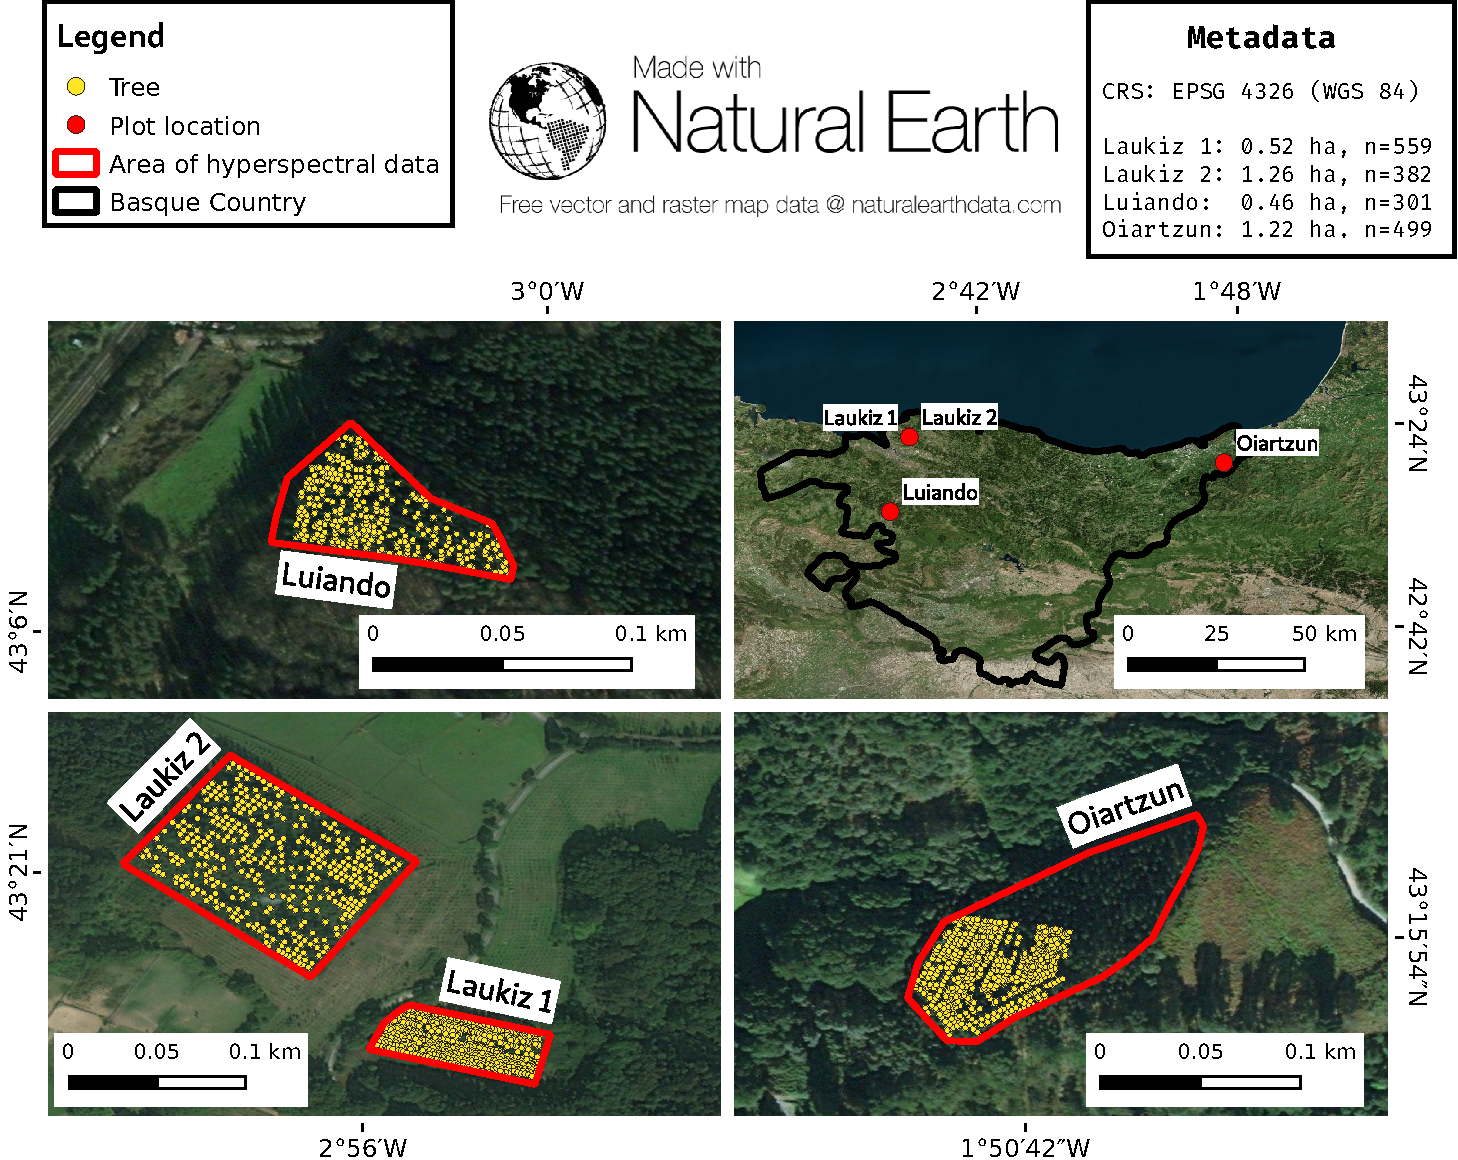
\includegraphics[width=\textwidth] {../03_figures/data/study_area_hyperspectral.pdf}}
		\caption{Information about the plot locations, the area of hyperspectral coverage and the number of trees per plot.}
		\label{fig:study_area}
	\end{center}
\end{figure}

% describe the hyperspectral data


\cite{Brenning2012}

% \begin{figure} [t!]
% 	\begin{center}
% 		\makebox[\textwidth]{\includegraphics[width=\textwidth] {../../04_figures/01_data/study_area.pdf}}
% 		\caption[Study area]{Spatial distribution of tree observations within the Basque Country, northern Spain, showing infection state by \textit{Diplodia sapinea}.}
% 		\label{fig: study_area}
% 	\end{center}
% \end{figure}

\subsection{Hyperspectral data}

The airborne hyperspectral data was acquired during two flight campaigns on September 28th and October 5th 2016, both around 12 am.
The images were taken by an AISAEAGLE-II sensor from the \ac{ICGC}.
All preprocessing steps (geometric, radiometric, atmospheric) have been conducted by \ac{ICGC}.

Additional information is provided in Table 1:

% parameter limits
\begin{table}[b!]
\centering
\caption[t]{Specifications of hyperspectral data.}
\begingroup\footnotesize
\begin{tabular}{ll}
	\\
	Characteristic         & Value                               \\
	\hline
	Geometric resolution   & 1 m                                 \\
	Radiometric resolution & 12 bit                              \\
	Spectral resolution    & 126 bands (404.08 nm - 996.31 nm)   \\
	Correction:            & Radiometric, geometric, atmospheric
\end{tabular}
\endgroup
\label{tab:hyperparameter_limits}
\end{table}



\section{Methods}

\subsection{Derivation of indices}

% link to PDF with veg indeces
All vegetation indices (90 total) suitable for the wavelength range of the hyperspectral data and offered by the \texttt{hsdar} package have been calculated.
Additionally, all possible \ac{NRI} were calculated from the data using the formula:

\begin{equation}
	NRI_{i,j} = \frac{b_{i} - b_{j}}{b_{i} + b_{j}}
\end{equation}

\noindent
where $i$ and $j$ are the respective band numbers.

%To account for geometric offsets, we calculated every index five times using a buffer from 1 - 5 meter around the centroid of the respective tree.
To account for geometric offsets, we used a buffer of 2 meters around the centroid of the respective tree.
The mean value of all pixels touched by the buffer was assigned as the final value for each index.
Missing values were removed from the mean value calculation.
In total, 7875 \ac{NRI}s have been calculated ($\frac{125*126}{2}$).
Some indices returned \texttt{NA} values for some observations and were removed from the dataset, leaving a total of 7471 indices that were available for all plots without missing values.
Note that due to the mass of variables we cannot state which indices in detail have been removed.

\subsection{Penalized regression}

The aim of this work was to find the indices that best explain defoliation within the plots.
We used penalized regression to account for the large amount of highly correlated predictor variables.
In a standard \ac{OLS} regression one of the assumptions is that the predictor variables should be independent when minimizing the \ac{RSS} \citep{Bare1981, Hastie2001}:

\begin{equation}
	RSS = \sum_{i=1}^{n} \left(y_{i} - \beta_{0} - \sum_{j=1}^{p} \beta_{j} x_{ij} \right) ^{2}
\end{equation}

where $\beta_{0}$ is the intercept, $\beta_{i}$ the coefficient, $x_{ij}$ the predictor variable and $y_{i}$ the response variable.

If this assumption is violated, regression coefficients can be highly biased.
They can even show the wrong sign and are very sensitive to adding new independent variables or data points to the model.
These points reduce the robustness and performance of \ac{OLS} regression when dealing with multicollinearity.
One approach to overcome these limitations is to penalize the coefficients.
This method leads to a substantial decrease in variance and better predictive performance compared to \ac{OLS} regression.
However, it also sacrifies the assumption of unbiased coefficients.
Hence, the resulting coefficients cannot be used for statistical inference but should be interpreted as a measure of variable importance.


\subsubsection{The ridge penalty}

In \ac{RR} (also called $\ell_{2}$ penalization) the assumption of unbiased coefficients is given up in favor of higher predictive accuracy and reduced variance \citep{Hastie2001}.
Coefficients are standardized and penalized for their size.
When minimizing the \ac{RSS}, \ac{RR} adds a penalization term $\lambda \sum_{j=1}^{p}\beta_{j}^{2}$ to the equation:

\begin{equation}
	RSS = \sum_{i=1}^{n} \left(y_{i} - \beta_{0} - \sum_{j=1}^{p} \beta_{j} x_{ij} \right) ^{2} + \lambda \sum_{j=1}^{p}\beta_{j}^{2}
\end{equation}

where $\lambda >= 0$ is a tuning parameter responsible for the magnitude of penalization.
To make the second term (usually referred to as the \textit{shrinkage penalty}) of this equation small, the coefficients $\beta_{j}$ need to become small.
Unlike to Lasso however, predictors are not removed from the final model and will always be $\beta_{j} >= 0$.
Hence, $\lambda$ has the effect of shrinking the coefficients when minimizing the \ac{RSS}.
For $\lambda = 0$, no penalization is done and standard \ac{OLS} applies \citep{James2013}.
The \textit{shrinkage penalty} is only applied to the coefficients and not to the intercept.
Also, while \ac{OLS} generates only one set of coefficient estimates, \ac{RR} will create multiple sets for every value of $\lambda$.
In summary, the advantage of \ac{RR} is based on the bias-variance tradeoff: For $\lambda\to\infty$, the flexibility of the fit is reduced leading to a decrease in variance of the coefficients but also introduces a (substantial) bias.
For $\lambda = 0$, the variance is high but coefficients are unbiased \citep{James2013}.

\subsubsection{The lasso penalty}

While the Ridge penalty $\lambda \sum_{j=1}^{p}\beta_{j}^{2}$ shrinks the coefficients, it does not exclude any predictor from the model by setting the coefficient to zero.
This is what the Lasso penalty (also called $\ell_{1}$) does: It works similar to a "best subset selection" approach by only keeping the most important variables in the model and reducing the coefficients of unimportant ones down to zero.
This is done by a different \textit{shrinkage penalty} $\lambda \sum_{j=1}^{p} \mid\beta_{j}\mid$ that is added to the \ac{OLS} term when minimizing the \ac{RSS}:

\begin{equation}
	RSS = \sum_{i=1}^{n} \left(y_{i} - \beta_{0} - \sum_{j=1}^{p} \beta_{j} x_{ij} \right) ^{2} + \lambda \sum_{j=1}^{p} \mid\beta_{j}\mid
\end{equation}

Subsequently, Lasso is performing variable selection and results in a sparse model that has the advantage of a simplied interpretability compared to Ridge models.
However, coeffcients are still biased due to penalization \citep{Hastie2001, James2013}.

\subsubsection{The elasticnet penalty}

The \textit{elasticnet penalty} combines both penalties Lasso and Ridge by weighting them with a parameter $\alpha$ that needs to be optimized.
It was introduced by \cite{Zou2005} with the idea to combine the advantages of both penalty terms.
The \textit{elasticnet penalty} is written as

\begin{equation}
	\lambda \sum_{j=1}^{p} \alpha\beta_{j}^{2} + (1 - \alpha) \mid\beta_{j}\mid
\end{equation}

where $\alpha$ weights the contribution of either the Lasso or Ridge penalty.
For $\alpha = 0.5$ both are weighted equally.
When $\alpha = 0$ only Ridge is used and for $\alpha = 1$ only Lasso applies \citep{Hastie2001}.

\subsection{Modeling}

\subsubsection{Selecting the best penalty}

As the introduced penalties behave different depending on the characteristics of the dataset, we first conducted a nested 10-fold spatial \ac{CV} to find the best method among those three.
The model comparison was applied to all of the four plots using \ac{RMSE} as the error measure.
For both the performance evaluation and hyperparameter tuning a spatial sampling using $k$-means clustering was used \citep{sperrorest}.
For the tuning, 200 random search iterations were used.
The limits of the tuning space for $\lambda$ were set to the internally calculated (data driven) limits of the R package \texttt{glmnet}.

\subsubsection{Extraction of the most important variables}

Next, we applied the winning method (\ac{RR}) on all plots.
Hyperparameter tuning of $\lambda$ for the full dataset was again done using a spatial sampling.
The ten highest coefficients (both positive and negative) were extracted and reported.

% parameter limits
\begin{table}[b!]
\centering
\caption[t]{10-fold 20-times repeated spatial \ac{CV} performances of lasso, ridge and elasticnet penalties on the plot level and the merged dataset using \ac{RMSE} as the error measure. Values show the overall mean and standard deviation at the repetition level.}
\begingroup\footnotesize
\begin{tabular}{llll}
	\\
	Plot/Penalty   & Lasso         & Ridge        & Elasticnet    \\
	\hline
	Laukiz 1       & 133.15 (4.66) & 86.71 (2.96) & 121.04 (4.15) \\
	Laukiz 2       & 91.93 (6.78)  & 29.73 (0.38) & 47.18 (13.70) \\
	Luiando        & 74.85         & 76.02        & 74.77         \\
	Oiartzun       & 327.93        & 106.65       & 260.38        \\
	Merged dataset & 56.88         & 55.88        & 56.76         \\
	\bottomrule
\end{tabular}
\endgroup
\label{tab:penalty_comparison}
\end{table}

\subsubsection{Linking variables to plot characteristics}

To interpret the outcomes of the models on a plot level, we linked the winning variables of each to dataset attributes that describe the underlying plot characteristics.
For example, a plot which a low tree density might inherit more information from the bare ground in the calculated indices while a plot with a very high tree density might in contrast contain information from multiple trees.
Also, the overall level of defoliation for the whole plot might possibly have an effect how well an index is able to describe the situation.

\subsubsection{Creation of a super model with all observations}

After the plot level analysis, we merged all observations into a single dataset and fitted another \ac{RR} model.
We used a block-level based spatial \ac{CV} for this setup.
For a total number of $m$ folds ($n$ = number of plots), every plot is once the test set while the training is done on the remaining ones.
This ensures that the test set is fully spatially independent from the training set.
Tuning was also performned on the block level within the training set on $n - 1$ folds using 200 random search iterations.
Due to the fixing of the indices on a plot level, varying those to use multiple repetitions is not possible.
The idea behind fitting a supermodel is that this model includes information from all plots rather than just from a single plot.
This may possibly reduce the predictive error and create a more robust model.

% Points to mention
% * All penalization methods are suited for different kinds of dataset structures
% * Find out which one works best on average and then use this method to create create models for prediction and variable importance

\section{Results}

\subsection{Plot characteristics}

Luiando shows the highest defoliation ($\bar{x} = 68.36 \%$) among the plots while Laukiz 2 is the healthiest ($\bar{x} = 17.73 \%$) (\autoref{fig:defol_boxplots}).
Laukiz 1 and Oiartzun both show a medium defoliation level around 50 \%.
Oiartzun consists mainly of trees that show either a very high level of defoliation ($70 \% <=$) or none at all.
Laukiz 1 shows an evenly distributed level of defoliation across the entire plot.

The high defoliation level of Luiando and Oiartzun is also visible in the spectral signatures of the plots (\autoref{fig:spectral_signatures}).
Both plots show lower mean reflectance values around the wavelength range 800 nm - 1000 nm compared to Laukiz 1 and Laukiz 2.
Oiartzun is almost completely missing the reflectance drop at around 815 nm that is visible for all other plots but instead shows a higher magnitude for the reflectance increase at around 920 nm.
Laukiz 2 shows a mean tree density of 62.51 m \autoref{fig:rmse_defol_dens}) while all other plots are more dense (34.35 (Laukiz 1), 33.77 (Luiando), 35.02 (Oiartzun)) (\autoref{fig:rmse_defol_dens}).

% defoliation boxplots
\begin{figure} [t!]
	\begin{center}
		\makebox[\textwidth]{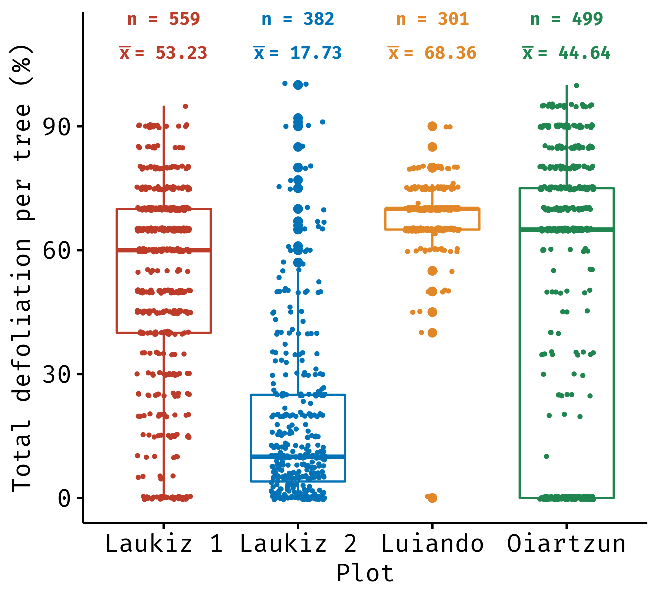
\includegraphics[width=0.7\textwidth] {../03_figures/results/boxplot_defol.pdf}}
		\caption{Descriptive statistics of the response variable \textit{defoliation}.}
		\label{fig:defol_boxplots}
	\end{center}
\end{figure}

% spectral signatures
\begin{figure} [t!]
	\begin{center}
		\makebox[\textwidth]{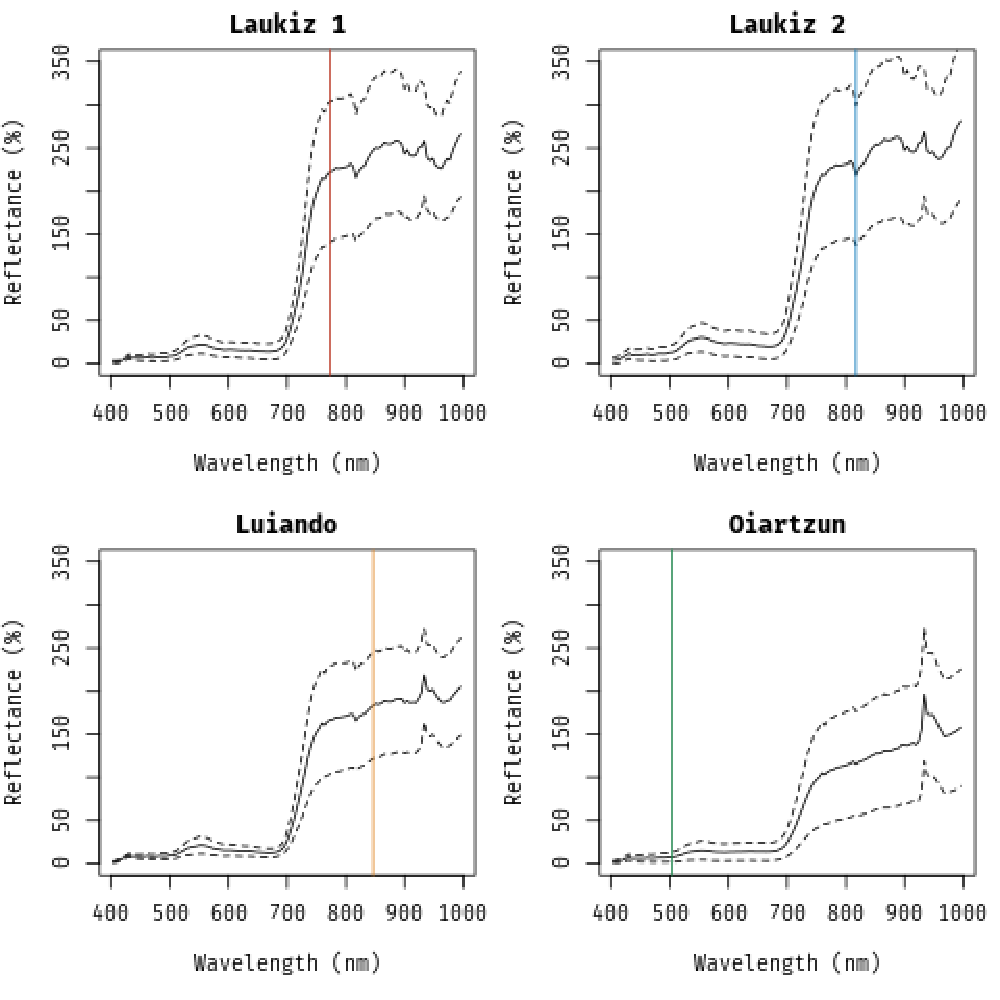
\includegraphics[width=\textwidth] {../03_figures/results/spectral_signatures.pdf}}
		\caption{Spectral signatures (mean and standard deviation) of each plot.
			The colored lines show the most important band for each plot, respectively: Band 80 (773nm, red), band 89 (817nm, blue), band 95 (846nm, orange), band 23 (503nm, green).}
		\label{fig:spectral_signatures}
	\end{center}
\end{figure}

\subsection{Predictive performance}

\begin{table}[t!]
\centering
\caption[t]{Predictive performance of \ac{RR} using the merged dataset (supermodel) and observations on a plot level only (single plot) with \ac{RMSE} as the error measure. The values for "merged dataset" correspond to the fold for which the respective plot was serving as the test set. For "single plot", the values correspond to the mean value of the SpCV at the repetition level (10 folds, 20 repetitions).}
\begingroup\footnotesize
\begin{tabular}{lll}
	\\
	Plot/Data & Merged dataset (Block CV) & Single plot (SpCV) \\
	\hline
	Laukiz 1  & 58.95                     & 89.89              \\
	Laukiz 2  & 27.94                     & 30.37              \\
	Luiando   & 69.72                     & 76.02              \\
	Oiartzun  & 58.09                     & 106.65             \\
	\bottomrule
\end{tabular}
\endgroup
\label{tab:supermodel_performance}
\end{table}

\ac{RR} shows the lowest error for three out of four plots (for Luiando \textit{elasticnet} shows a slightly better performance) (\autoref{tab:penalty_comparison}).
The magnitude of difference for \ac{RR} compared to the other penalties for the plots in which \ac{RR} showed the best performance ranges between XX and XX percent.
For the merged dataset, all penalties show a similar mean predictive performance that outperform all single plot models besides the Laukiz 2 model.

When comparing the mean predictive performance of the plot level model against the performance of the super model at the plot level (when the respective plot served as the test set), the supermodel also outperforms the Laukiz 2 model (27.94 vs 30.37 RMSE) (\autoref{tab:supermodel_performance}).

The worst performance of the supermodel on the fold level is reported for Luiando (69.72 RMSE) while for the single plot models Oiartzun shows the highest error (106.65 RMSE).

% rmse vs defol and point dens
\begin{figure} [b!]
	\begin{center}
		\makebox[\textwidth]{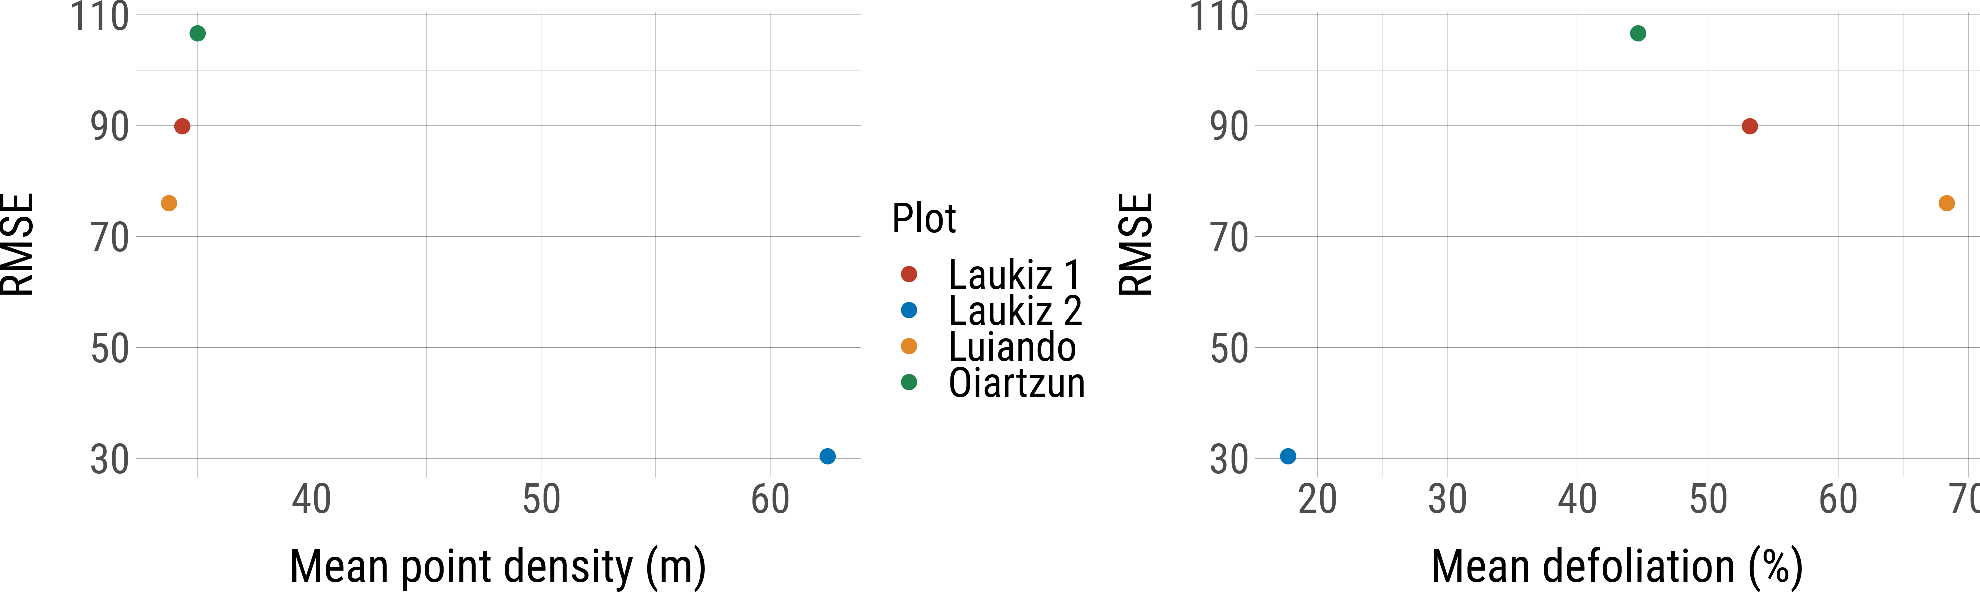
\includegraphics[width=\textwidth] {../03_figures/results/mean-defol_mean-point-dens.pdf}}
		\caption{RMSE vs. mean defoliation and point density}
		\label{fig:rmse_defol_dens}
	\end{center}
\end{figure}

\section{Discussion}

\subsection{Index derivation}

The exact number of contributing pixels of an index cannot be determined as it depends on the location of the tree within the pixel grid.
If a tree is located at the border of a pixel, the same buffer (e.g. 3 m) will include more pixels than if the point is located at the center of a pixel.
Also, if a tree is located at the border of the image data, some directions of the buffer may not contain values.

\subsection{Variable importance}

% variable importance
\begin{table}[b!]
\centering
\caption[t]{The ten highest coefficient estimates for every plot and the merged dataset.}
\begingroup\footnotesize
\begin{tabular}{lllll}
	\\
	Laukiz 1           & Laukiz 2           & Luiando             & Oiartzun            & All Plots          \\
	\hline
	b80-b77 (0.0089)   & b89-b84 (0.0093)   & b95-b93 (1.5e-36)   & b23-b18 (-0.0090)   & b78-b77 (0.058)    \\
	b81-b77 (0.0079)   & b89-b87 (0.0086)   & b109-b106 (1.4e-36) & b23-b19 (-0.0074)   & b115-b113 (0.054)  \\
	b78-b77 (0.0079)   & b89-b88 (0.0086)   & b92-b95 (1.4e-36)   & b99-b98 (0.0073)    & b82-b77 (0.052)    \\
	b77-b76 (-0.0078)  & b108-b104 (0.0084) & b114-b6 (-1.2e-36)  & b23-b20 (-0.0070)   & b79-b77 (0.049)    \\
	b79-b77 (0.0077)   & b89-b85 (0.0083)   & b96-b93 (1.2e-36)   & b10-b8 (-0.0063)    & b80-b77 (0.049)    \\
	Datt3 (-0.71)      & b92-b84 (0.0083)   & b116-b6 (-1.2e-36)  & b102-b98 (0.0062)   & b81-b77 (0.049)    \\
	b41-b25 (0.0070)   & b89-b83 (0.0081)   & b114-b5 (-1.2e-36)  & b124-b115 (0.0062)  & b81-b78 (-0.048)   \\
	b116-b113 (0.0068) & b89-b86 (0.0080)   & b115-b114 (1.2e-36) & b23-b15 (-0.0060)   & b124-b115 (-0.047) \\
	b82-b77 (0.0068)   & b92-b88 (0.0080)   & b95-b91 (1.1e-36)   & b126-b115 (-0.0060) & b23-b20 (-0.047)   \\
	b77-b75 (-0.0068)  & b108-b96 (0.0079)  & b114-b8 (-1.1e-36)  & b118-b115 (-0.0059) & b80-b78 (-0.046)   \\
	\bottomrule
\end{tabular}
\endgroup
\label{tab:variable-importance}
\end{table}

\section*{References}

\bibliography{Biblio_hyperspectral}

\end{document}
